\documentclass{article}
\usepackage{avremu}
\usepackage{listings}
\usepackage{hyperref}
\usepackage{filecontents}
\usepackage{tcolorbox}
\usepackage{ydoc}

\def\fileversion{v0.1}
\def\filedate{2014/10/09}

\makeatletter
\def\cmd#1{\cs{\expandafter\cmd@to@cs\string#1}}
\def\cmd@to@cs#1#2{\char\number`#2\relax}
\DeclareRobustCommand\cs[1]{\texttt{\char`\\#1}}
\makeatother

\begin{filecontents*}{hello-world.c}
#include <avr/io.h>

int
main(void)
{
  char *str = "Hello World!";
  char *p = str;
  while (*p) {
    UDR = *p++;
  }
  asm  volatile ("break;");
}
\end{filecontents*}

\title{The \texttt{avremu} Package}
\author{Christian Dietrich\\
\url{stettberger@dokucode.de}\\
\url{https://gitlab.brokenpipe.de/stettberger/avremu}}

\begin{document}

\maketitle

\begin{tcolorbox}
  \lstinputlisting[language=C]{hello-world.c}
  \tcblower
  \begin{lstlisting}[language=TeX]
\avrloadc{hello-world.c}
\avrrun
UDR='\avrUDR' in \avrinstrcount\ instructions
\end{lstlisting}
\end{tcolorbox}
\begin{tcolorbox}
\avrloadc{hello-world.c}\avrrun
UDR='\avrUDR' in \avrinstrcount\ instructions
\end{tcolorbox}


\LaTeX\ is known as a typesetting system. But the underlying \TeX\ system is a powerful macro
processor. In fact, TeX is a Turing-complete programming language. \TeX\ can compute anything that
is computable. Computeability is a concept from theoretical computer science. After visiting a
theoretical computer-science course, you will know that there are things that cannot be solved by a
machine. Never. Look out for the halting problem. 

This package does contain an \emph{CPU emulator} for the 8-bit microcontroller platform Atmel AVR, more
precisely it implements the instruction-set architecture of the \texttt{ATmega8}.

\begin{tcolorbox}
\begin{lstlisting}[language=TeX]
\avrloadc{mandelbrot.c}
\avrrun

\avrdrawppm{mandelbrot.ppm}
\immediate\write18{convert mandelbrot.ppm mandelbrot.png}
  
\includegraphics[width=\linewidth]{mandelbrot.png}
\end{lstlisting}
  \tcblower
  This picture (250x250) took 44 hours to render. The source code can be found in the test-suite
  directory under mandelbrot.c.\\

  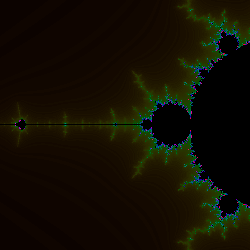
\includegraphics[width=\linewidth]{imgs/mandelbrot-250x250}
\end{tcolorbox}

\section{Provided Commands}

\DescribeMacro{\avrloadihex}{\meta{filename}}
Load an Intel HEX formatted image of the flash into the code memory of the AVR
emulator. Additionally the state of the AVR emulator is set back to zero.

\DescribeMacro{\avrloadc}[\meta{compiler options}]{\meta{filename}}
Requires \verb|--shell-escape|. Compiles C source code file with \verb|avr-gcc| and the given
compiler options. The default compiler option set is \verb|-mmcu=atmega8 -Os|. The resulting
\texttt{.elf} file is transformed to an Intel HEX file and loaded into the code memory of the
emulator.

\DescribeMacro{\avrrun}
Run the emulator until a \textbf{break} instruction occurs.

\DescribeMacro{\avrstep}[\meta{steps}=1]
Run the emulator for N instructions. The default is a single step. The stepping does automatically
end, if a \textbf{break} instruction is executed.

\DescribeMacro{\avrinstrcount}
Expands to the number of executed instructions.

\DescribeMacro{\avrsinglestep}
Starts an interactive single-stepping mode, which was mainly used for implementing the emulator.

\DescribeMacro{\usravremulibrary}{\meta{list of libraryies}}

\subsection{Access to the Serial Console}
If the program write to the \verb|UDR| IO register, the emulator catched those characters in an
internal buffer.

\DescribeMacro{\avrUDR}
Expands to the internal UDR buffer.

\DescribeMacro{\avrUDRclear}
Clears the internal UDR buffer.

\subsection{Draw Library}
\DescribeMacro{\useavremulibrary}{avr.draw}

See source/test-suite/mandelbrot.c for more details.

\section{Implementation Details}
Read the source.
\end{document}

%%% Local Variables: 
%%% mode: latex
%%% TeX-master: t
%%% End: 
